\documentclass{article}
\usepackage{tikz}
\usepackage{adjustbox}

\begin{document}

\begin{center}
    \textbf{Mission Display:}
\end{center}

\begin{adjustbox}{center}
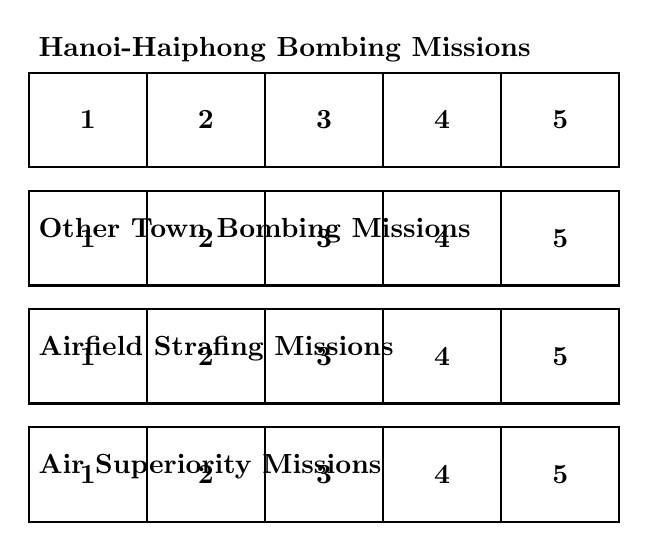
\begin{tikzpicture}
    % Define box size
    \def\boxwidth{1.5}
    \def\boxheight{1.2}
    \def\spacing{0.5} % Space between text and boxes


    % Categories
    \node[anchor=west] at (0.0, 0.3) {\textbf{Hanoi-Haiphong Bombing Missions}};
    \node[anchor=west] at (0.0, -2) {\textbf{Other Town Bombing Missions}};
    \node[anchor=west] at (0.0, -3.5) {\textbf{Airfield Strafing Missions}};
    \node[anchor=west] at (0.0, -5) {\textbf{Air Superiority Missions}};

    % Draw the boxes for each category
    \foreach \y in {0, -1.5, -3, -4.5} {
        \foreach \x in {0,1,2,3,4} {
            \draw[thick] (\x*\boxwidth, \y) rectangle (\x*\boxwidth + \boxwidth, \y-\boxheight);
            \node at (\x*\boxwidth + 0.75, \y-0.6) {\textbf{\the\numexpr\x+1}};
        }
    }
\end{tikzpicture}
\end{adjustbox}

\end{document}

